\section{Substrati usati, meccanismi di reazione e risultati sperimentali}

\subsection{Alchini funzionalizzati con alogenuri}
\subsubsection{Sililformilazione}\begin{frame}\frametitle{Alchini funzionalizzati con alogenuri}\framesubtitle{Sililformilazione}
Il risultato della {\bf sililformilazione di alchini funzionalizzati con buoni gruppi uscenti} dipende dalla posizione di questi:
\begin{itemize}
 \item sostituenti in alfa al triplo legame: si ha decomposizione; 
 \item sostituenti in posizioni più lontane non sono problematici per la sililformilazione.
\end{itemize}


\end{frame}

%%%%%%%%%%%%%%%%%%%%%%%%%%%%%%%%%%%%%%%%%%%%%%%%%%%%%%%%%%%%%%%%%%%%
\logo{}
\subsubsection{Desililazione}\begin{frame}\frametitle{Alchini funzionalizzati con alogenuri}\framesubtitle{Desililazione}
Nella {\bf desililazione con migrazione} del gruppo aromatico si ha un {\bf effetto importante} sulla reattività da parte di {\bf alogenuri e tosilati}.
\begin{columns}
\column{0.5\linewidth}


In dipendenza dalla posizione dell'alogenuro nella catena alifatica del $\beta$-sililalchenale si può avere la {\bf formazione di cicli secondo diversi meccanismi}.  
\column{0.5\linewidth}\begin{figure}{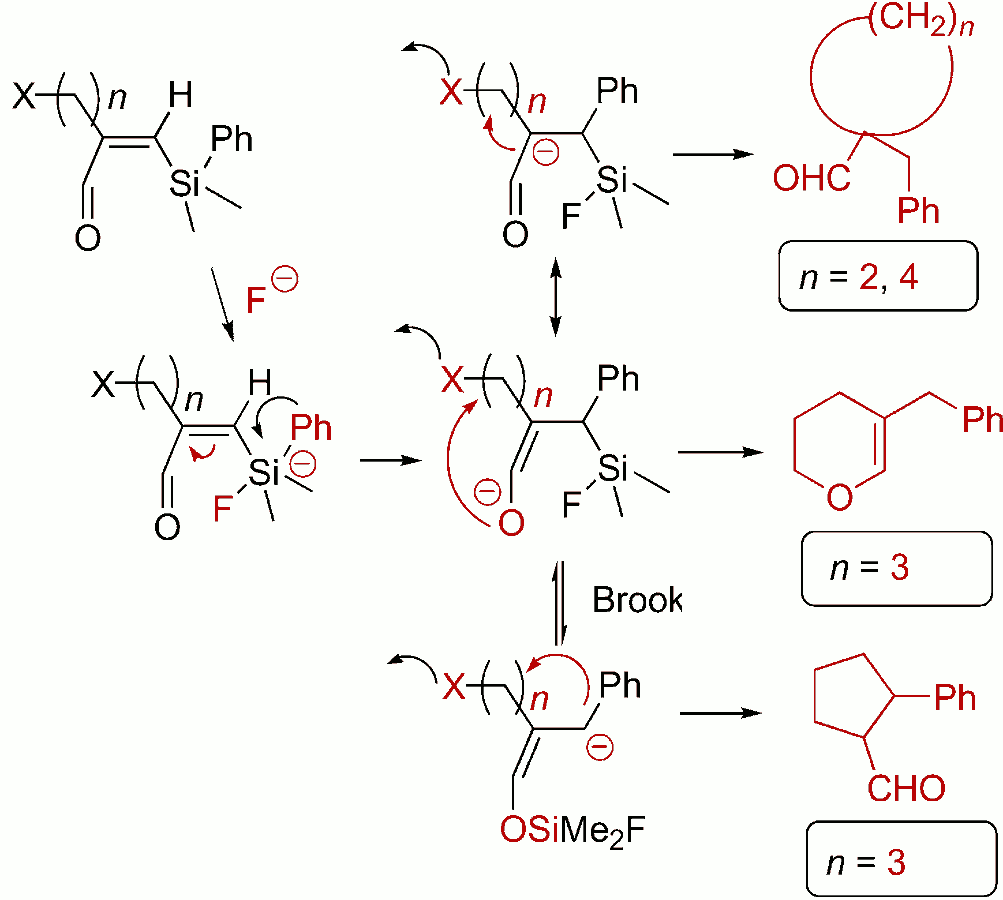
\includegraphics[width=1\textwidth]{img/substrati/alogenuri.png}}\end{figure}

\end{columns}
\end{frame}
\logo{
\includegraphics[width=0.07\paperwidth]{img/snslogo.png}}

\begin{frame}\frametitle{Alchini funzionalizzati con alogenuri}\framesubtitle{Desililazione}
Anche in presenza di gruppi uscenti non ottimi come il cloruro si ha una prevalenza della formazione di cicli sul prodotto lineare 1-benzilaldeide. {\bf In ogni caso si formano anelli a 3, 5 e 6 membri}.
 \begin{figure}{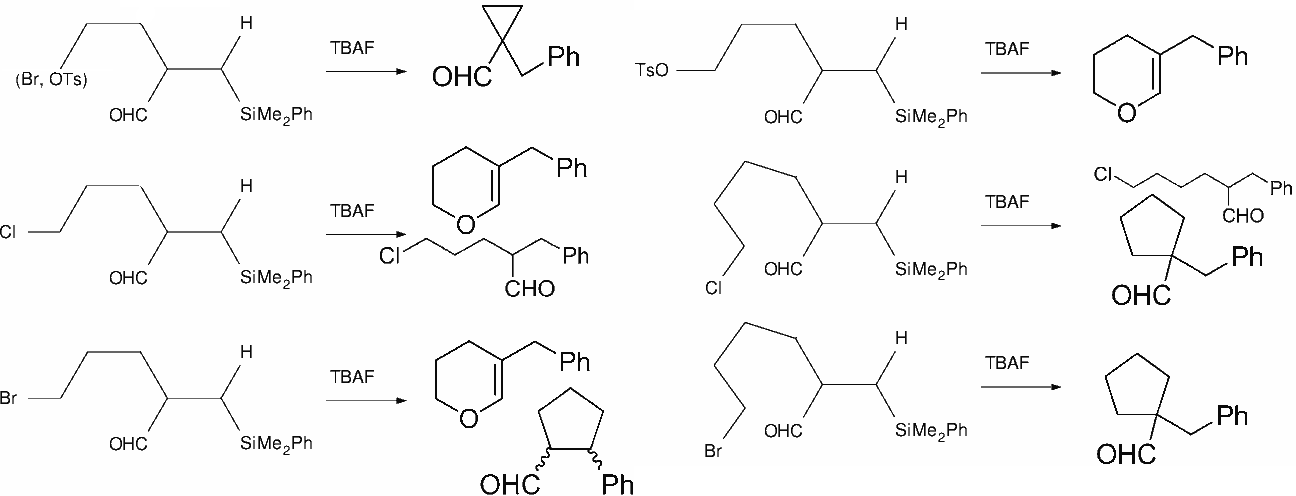
\includegraphics[width=1\textwidth]{img/substrati/alogenuri3.png}}\end{figure}

\end{frame}



%%%%%%%%%%%%%%%%%%%%%%%%%%%%%%%%%%%%%%%%%%%%%%%%%%%%%%%%%%%%%%%%%%%%

\subsection{Ammine propargiliche}
\subsubsection{Sililformilazione}\begin{frame}\frametitle{Ammine propargiliche}\framesubtitle{Sililformilazione}
La {\bf sililformilazione di ammine} propargiliche va a buon fine se l'{\bf ammina è protetta come tosilammide} (l'ammina libera potrebbe avvelenare il catalizzatore).
\begin{figure}{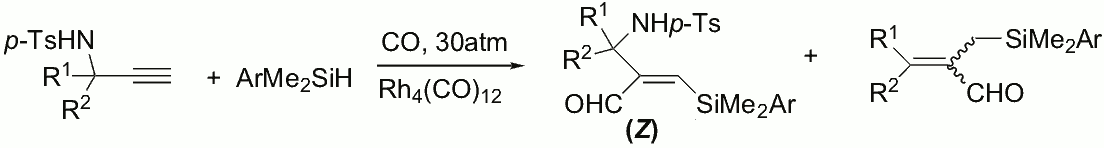
\includegraphics[width=0.95\textwidth]{img/substrati/ammine-sililform.png}}\end{figure}
Si hanno i {\bf prodotti secondari} mostrati in figura (probabilmente secondo un meccanismo in cui una seconda molecola di silano dà idrosililazione 1,4 del gruppo aldeidico nel $\beta$-sililalchenale e quindi eliminazione di una silanammide).


\end{frame}

%%%%%%%%%%%%%%%%%%%%%%%%%%%%%%%%%%%%%%%%%%%%%%%%%%%%%%%%%%%%%%%%%%%%

\subsubsection{Desililazione di $\beta$-sililalchenali}\begin{frame}\frametitle{Ammine propargiliche}\framesubtitle{Desililazione di $\beta$-sililalchenali}
\begin{columns}
\column{0.55\linewidth}
Su $\beta$-sililalchenali aventi in posizione $\alpha$ un {\bf gruppo tosilammide} (o un altro buon gruppo uscente) la desililazione avviene con {\bf eliminazione} della tosilammide per ottenere una 2-metilaril-2-alchenale.

Si ha preferenzialmente il prodotto più stabile E.

\column{0.45\linewidth}\begin{figure}{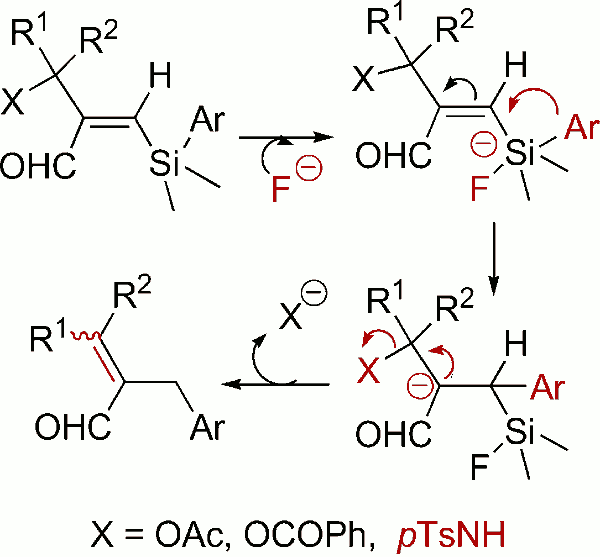
\includegraphics[width=1\textwidth]{img/substrati/ammine-desilil2.png}}\end{figure}
\end{columns}

\end{frame}

\subsubsection{Sililcarbociclizzazione}\begin{frame}\frametitle{Ammine propargiliche}\framesubtitle{Sililcarbociclizzazione}
In presenza di una {\bf base forte} (è stata impiegata una base organica ingombrata: DBU (1,8-Diazabiciclo[5.4.0]undec-7-ene)) {\bf la sililformilazione porta alla formazione di $\beta$-lattami}. 

Sembra che la base sia necessaria per spezzare il legame N--H.
\begin{figure}{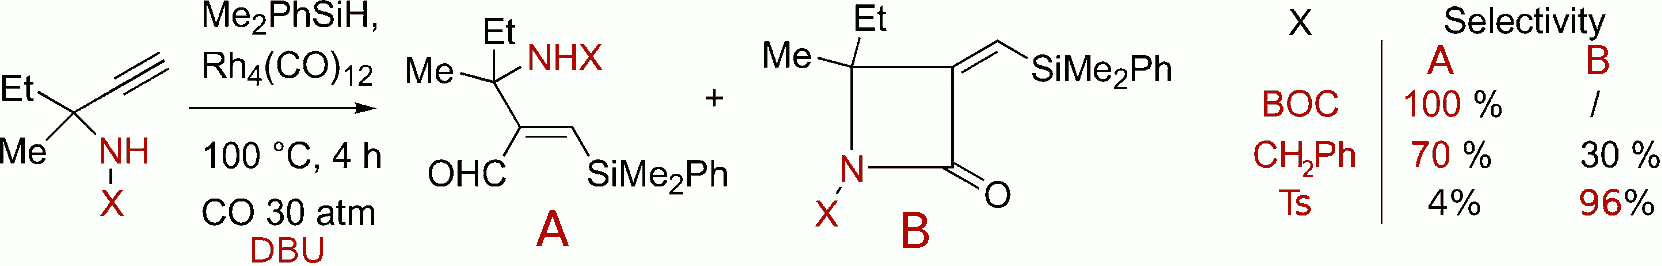
\includegraphics[width=1\textwidth]{img/substrati/ammine-cicliz.png}}\end{figure}
\pause
Contrariamente alla sililformilazione (favorita da alchini non ramificati) la {\bf sililcarbociclizzazione avviene bene solo se impiegata su alchini completamente sostituiti in posizione propargilica}.

\end{frame}

%%%%%%%%%%%%%%%%%%%%%%%%%%%%%%%%%%%%%%%%%%%%%%%%%%%%%%%%%%%%%%%%%%%%
\logo{}
\subsubsection{Desililazione di $\alpha$-sililmetilene $\beta$-lattami}\begin{frame}\frametitle{Ammine propargiliche}\framesubtitle{Desililazione di $\alpha$-sililmetilene $\beta$-lattami}
\begin{columns}
\column{0.6\linewidth}
Su $\alpha$-sililmetilene $\beta$-lattami la {\bf desililazione} con migrazione del gruppo aromatico avviene con {\bf buone rese} in 3-metilaril-$\beta$-lattame e alte diastereoselettività a favore del prodotto E più stabile.

\column{0.4\linewidth}
\vskip -13pt
\begin{figure}{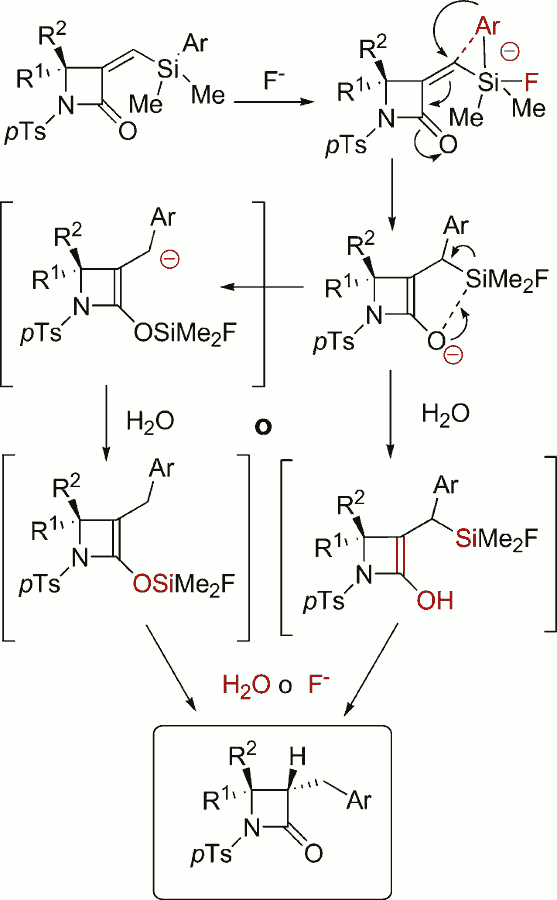
\includegraphics[width=1\textwidth]{img/substrati/ammine-cicl-desilil.png}}\end{figure}
\end{columns}
 
\end{frame}

\logo{
\includegraphics[width=0.07\paperwidth]{img/snslogo.png}}

%%%%%%%%%%%%%%%%%%%%%%%%%%%%%%%%%%%%%%%%%%%%%%%%%%%%%%%%%%%%%%%%%%%%
\diapo{Estensioni}
Una reattività simile alle ammine propargiliche si ottiene trattando alcoli propargilici ed omopropargilici:

 è possibile ottenere $\beta$ e $\gamma$ lattoni aventi in posizione 3 dei metilarili.
\begin{figure}{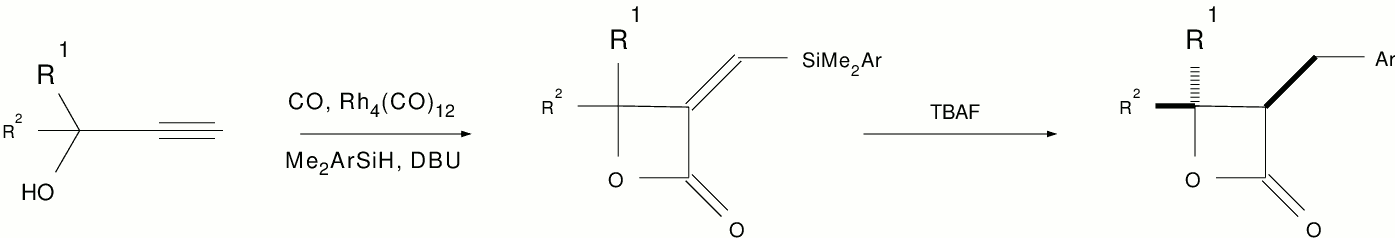
\includegraphics[width=1\textwidth]{img/substrati/alcol-tutto.png}}\end{figure}

     \end{frame}

%%%%%%%%%%%%%%%%%%%%%%%%%%%%%%%%%%%%%%%%%%%%%%%%%%%%%%%%%%%%%%%%%%%%

\subsection{Appendice: Alcoli propargilici}
\subsubsection{Sililformilazione}\begin{frame}\frametitle{Alcoli propargilici}\framesubtitle{Sililformilazione}
La {\bf sililformilazione di alcoli propargilici} in assenza di base avviene con {\bf buone rese}. 

A differenza delle precedenti sililformilazioni si ottengono diastereoselettività minori a causa della produzione del prodotto E in quantità dal 4 al 20\%. 
\begin{figure}{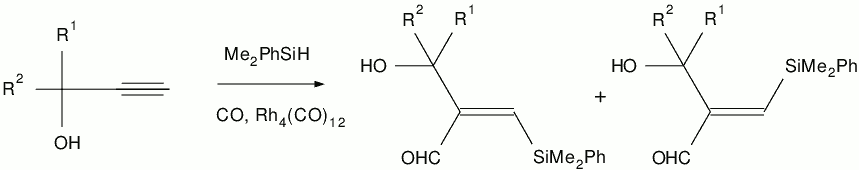
\includegraphics[width=0.9\textwidth]{img/substrati/alcol-sililform.png}}\end{figure}

\end{frame}
\logo{}
%%%%%%%%%%%%%%%%%%%%%%%%%%%%%%%%%%%%%%%%%%%%%%%%%%%%%%%%%%%%%%%%%%%%
\subsubsection{Desililazione di $\beta$-sililalchenali}\begin{frame}\frametitle{Alcoli propargilici}\framesubtitle{Desililazione di $\beta$-sililalchenali}
\begin{columns}
\column{0.5\linewidth}
Durante la {\bf desililazione} indotta da fluoruri si ha {\bf eliminazione} del gruppo OH alcolico.

Questo diviene un buon gruppo uscente a causa dell'alta affinità con il silicio.
\column{0.5\linewidth}
\begin{figure}{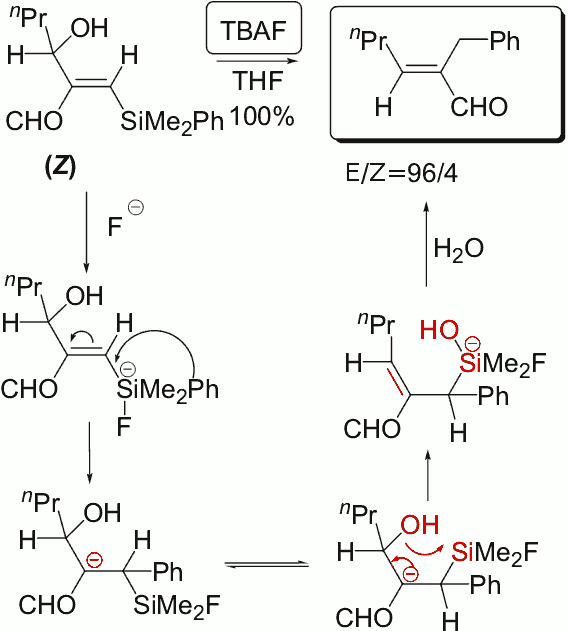
\includegraphics[width=1\textwidth]{img/substrati/alcol-desilil.png}}\end{figure}
     \end{columns}     
  \end{frame}\logo{
\includegraphics[width=0.07\paperwidth]{img/snslogo.png}}

\subsubsection{Sililcarbociclizzazione}\begin{frame}\frametitle{Alcoli propargilici}\framesubtitle{Sililcarbociclizzazione}
Nella {\bf sililformilazione di alcoli} propargilici in presenza di base DBU si ottengono rese in $\beta$-lattoni dipendenti dal substrato:
\begin{itemize}
 \item su alcoli propargilici {\bf primari} si ottiene solo {\bf sililformilazione};
 \item su alcoli {\bf secondari} si ottiene una {\bf miscela} di prodotti (a meno di usare sul silano aromatici ingombrati in orto);
\begin{figure}{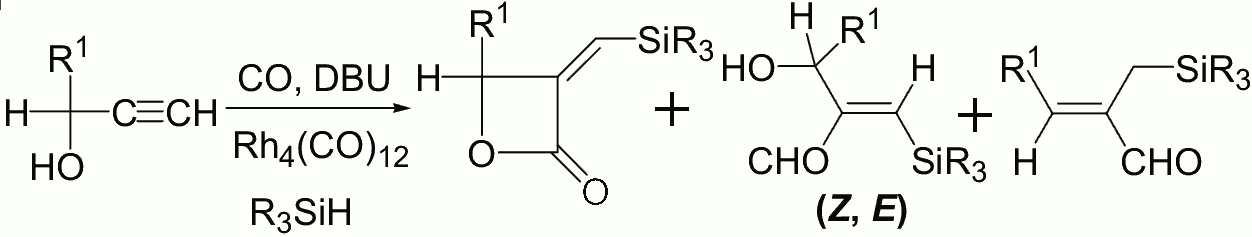
\includegraphics[width=0.7\textwidth]{img/substrati/alcol-secondari.png}}\end{figure}
 \item su alcoli {\bf terziari} alifatici si hanno {\bf buone rese} in $\beta$ lattoni;
 \item sul 2-fenil-3-butin-2-olo si hanno miscele di prodotti (alle alte temperature di reazione il lattone decompone con perdita di \ce{CO2}, a temperature più basse di può ottenere il lattone).
\end{itemize}
\end{frame}



%%%%%%%%%%%%%%%%%%%%%%%%%%%%%%%%%%%%%%%%%%%%%%%%%%%%%%%%%%%%%%%%%%%%
\subsubsection{Desililazione di $\alpha$-sililmetilene $\beta$-lattoni}\begin{frame}\frametitle{Alcoli propargilici}\framesubtitle{Desililazione di $\alpha$-sililmetilene $\beta$-lattoni}
                                                             La {\bf desililazione} con migrazione del gruppo aromatico {\bf procede bene con ogni lattone} trattato (tranne il 3-benzil-4-fenil-4-metil-ossetan-2-one che aveva già dato problemi di decomposizione nella sililcarbociclizzazione).

La desililazione è risultata altamente {\bf diastereoselettiva} permettendo di ottenere prodotti con i sostituenti più ingombranti in trans.
\begin{figure}{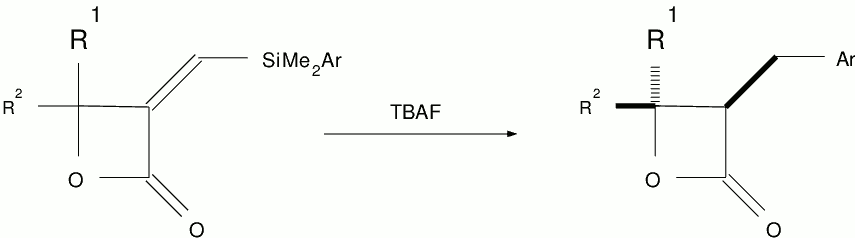
\includegraphics[width=0.85\textwidth]{img/substrati/alcol-desililcicl.png}}\end{figure}
\end{frame}

